To develop a suitable model based controller, the developed non-linear model should first be validate. This is done using a planar 2 degree-of-freedom soft robot. This robot has a translational and rotational degree of freedom. Rotation is only dependent on the difference in bellow length, not absolute bellow length. To measure rotation, an Inertial Measurement Unit (IMU) is connected at the tip of the robot. The position of the bellows can be tracked with an optical tracking system. From this data, elongation and curvature of each individual bellow can extracted. This allows validation of the dynamic model.


\section{Experimental set-up}


\subsection{Inertial Measurement Unit (IMU)}

\subsection{Pixy 2}

\subsection{Pressure sensor}


\subsection{Simplified Inverse Kinematics}


\begin{figure}[H]
    \centering
    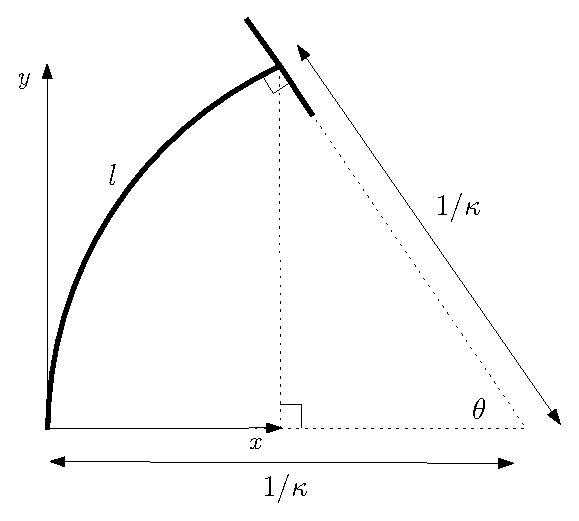
\includegraphics[width = 0.5\textwidth]{Figures/Chapter5/fbdkinematics.eps}
    \caption{Schematic drawing of the actuator to determine mapping from configuration space to task space}
    \label{fig:my_label}
\end{figure}


\begin{equation}
    \theta = l \kappa
\end{equation}


\begin{equation}
    y = \frac{1}{\kappa}\sin(l \kappa)
\end{equation}

\begin{equation}
    x = \frac{1}{\kappa}[1-\cos(l \kappa)]
\end{equation}




\section{Simulation model}





%\textbf{Assumptions}
%\begin{itemize}
%    \item The actuator is symmetrical, curvature equal but negative in when bellow is pressurized
%    \item Out of plane motion is negligible small
%    \item Constant curvature approach captures the kinematics well when neglecting the effect of gravity 
%\end{itemize}



